\documentclass[letter,11pt]{article}

\usepackage[spanish,es-nodecimaldot]{babel}
\usepackage[utf8]{inputenc}

\usepackage{lmodern}
\usepackage[T1]{fontenc}
\usepackage{textcomp}

\usepackage{framed}
\usepackage[svgnames]{xcolor}
\colorlet{shadecolor}{Gainsboro!50}

\usepackage[labelfont=bf]{caption}
\usepackage[shortlabels]{enumitem}
\usepackage{graphicx}
\usepackage{pstricks}

\usepackage{anysize}
\marginsize{3cm}{2cm}{2cm}{3cm}

\usepackage{url}
\usepackage{siunitx}
\usepackage{amsmath}
\usepackage{array}

\usepackage{caption}
\newcommand{\source}[1]{\vspace{-11pt} \caption*{\small{\textbf{Nota:} {#1}}}}

\usepackage{fancyhdr}
\usepackage{lastpage}
\pagestyle{fancy}
\fancyhf{}
\fancyhead[LE,RO]{Laboratorio de Física Básica II}
\fancyfoot[CO,CE]{\thepage\ de \pageref{LastPage}}

\special{papersize=215.9mm,279.4mm}

\usepackage[
    pdfauthor={Carlos Eduardo Caballero Burgoa},%
    pdftitle={Laboratorio de Física Básica II},%
    pdfsubject={Efecto Doppler},%
    colorlinks,%
    citecolor=black,%
    filecolor=black,%
    linkcolor=black,%
    urlcolor=black,
    breaklinks]{hyperref}
\usepackage{breakurl}

\newcommand{\blankpage}{
\newpage
\thispagestyle{empty}
\mbox{}
\newpage
}

\renewcommand{\arraystretch}{1.2}

\title{Informe 7: Efecto \emph{Doppler}}
\author{Carlos Eduardo Caballero Burgoa \\
    \small{\href{mailto:200201226@est.umss.edu}{200201226@est.umss.edu}}
}
\date{\today}

\begin{document}

\maketitle
\begin{center}
    \textbf{Grupo}: J2\\
    \textbf{Docente}: Ing. Milka Mónica Torrico Troche\\
    \textbf{Carrera}: Ing. Electromecánica
\end{center}

\begin{abstract}
Este documento detalla el experimento realizado en simulador para hallar la
relación funcional entre los diferentes casos posibles del efecto
\emph{Doppler}, además del hallar el valor de la velocidad del sonido en el
medio; para esto se realizó la medición de las velocidades y frecuencias, tanto
de un emisor de onda sonora como de un receptor; posteriormente se calculó las
relaciones funcionales con el método de mínimos cuadrados y finalmente se
determinó el valor de la velocidad del sonido, resultando ser: $343 [m/s]$.
\end{abstract}

\section{Introducción}

\begin{figure}
\centering
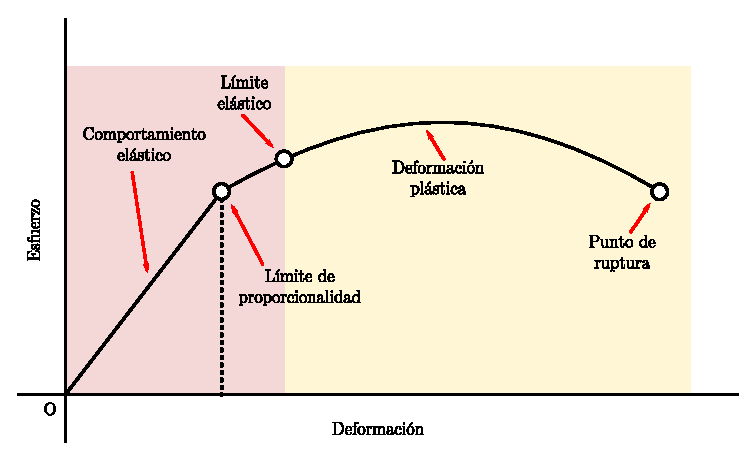
\includegraphics[width=0.68\textwidth]{resources/f1.eps}
\caption{Emisor de sonido y receptor en movimiento relativo.}
\label{figura1}
\source{Elaboración propia.}
\end{figure}

Cuando un emisor y un receptor de ondas sonoras están en movimiento relativo con
respecto al medio en el cual se propagan (\textbf{Figura \ref{figura1}}), la
frecuencia de las ondas recibidas es diferente de la frecuencia de las ondas
emitidas. Este fenómeno, descrito por primera vez por el científico austriaco
del siglo XIX \emph{Christian Doppler} \cite{Young&Freedman}.

Para analizar ese fenómeno, solo se considerará el caso especial en que las
velocidades del emisor y el receptor se encuentran a lo largo de la linea que
los une.

Se consideran tres posibles casos.

\subsection{Receptor en movimiento y emisor estacionario}

\begin{figure}
\centering
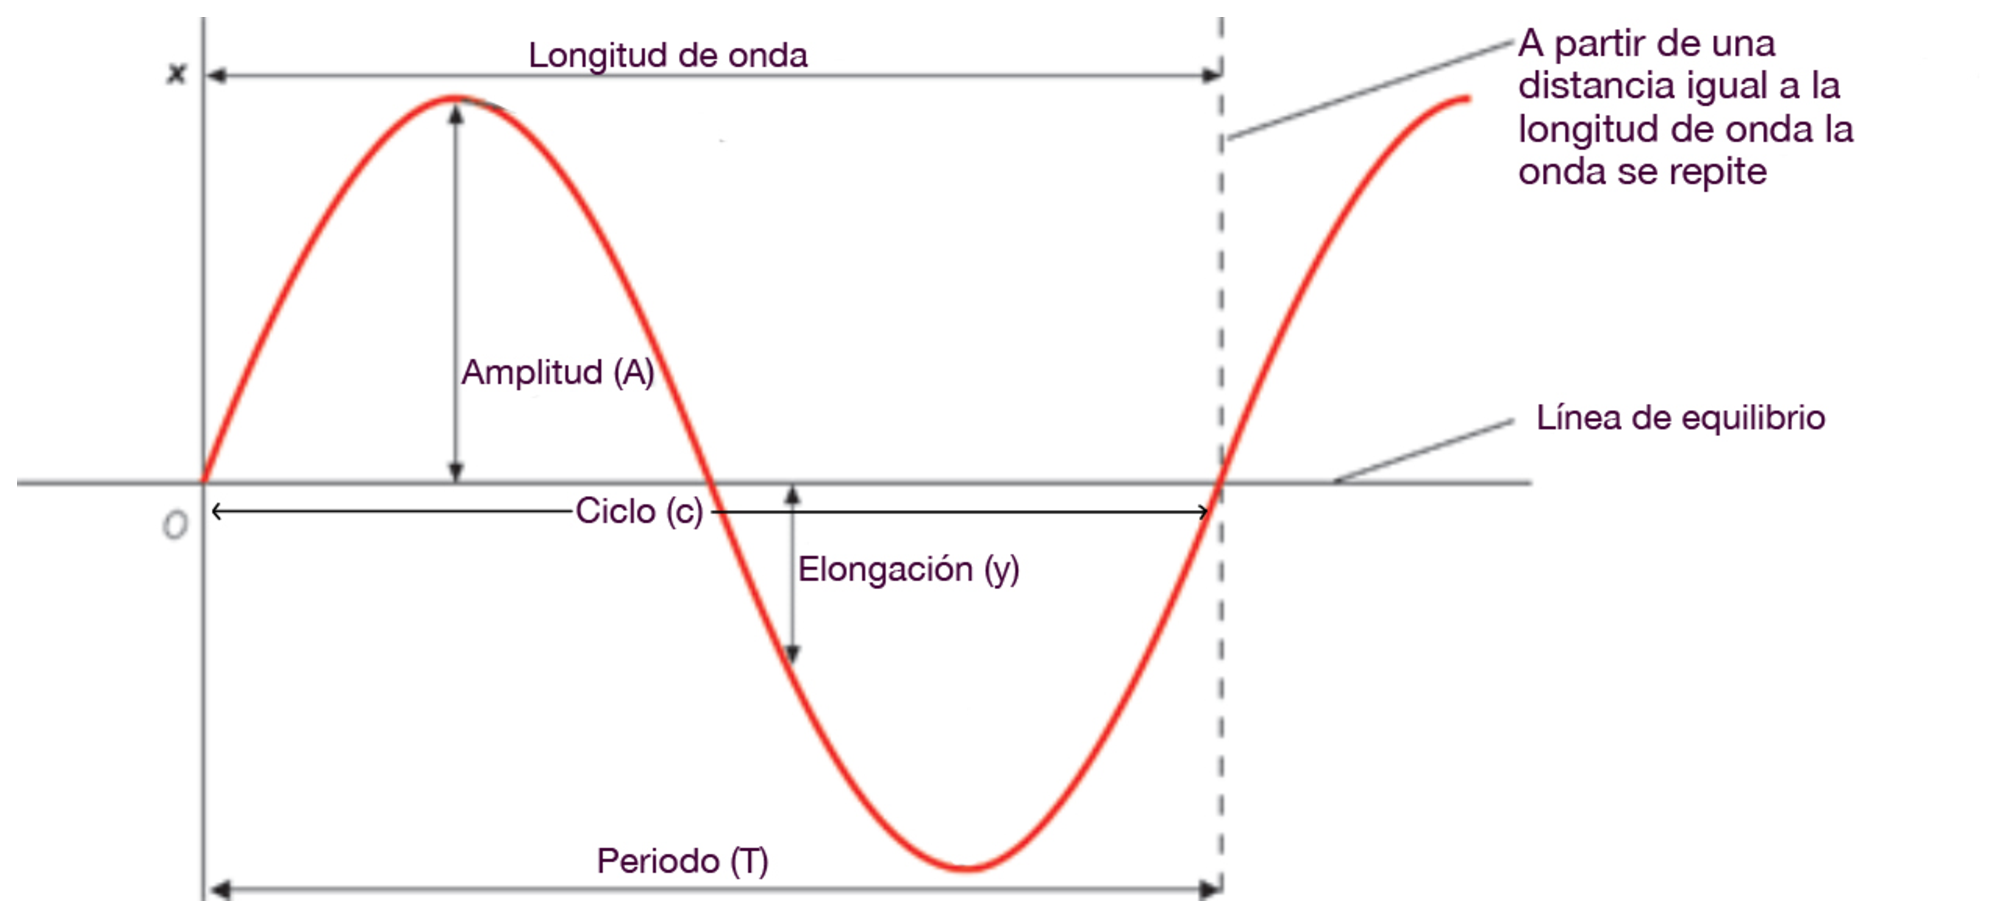
\includegraphics[width=0.68\textwidth]{resources/f2.eps}
\caption{Receptor en movimiento y emisor estacionario.}
\label{figura2}
\source{Elaboración propia.}
\end{figure}

Sea un receptor ($R$) que se mueve con velocidad ($v_R$) alejándose de un emisor
estacionario ($E$) como en la \textbf{Figura \ref{figura2}}. El emisor emite una
onda sonora con frecuencia ($f_E$) y longitud de onda ($\lambda = v/f_E$).

La rapidez de la onda sonora se acerca al receptor en movimiento con una rapidez
de propagación relativa igual a: $(v - v_R)$.

Por tanto la frecuencia que el receptor capta es:

\begin{equation*}
    f_R = \frac{v - v_R}{\lambda}
        = \frac{v - v_R}{v / f_E}
        = \left(\frac{v - v_R}{v}\right)\, f_E
\end{equation*}
\begin{equation}
    f_R = \left(1 - \frac{v_R}{v}\right)\, f_E
\end{equation}
\vspace{0.10cm}

Desarrollando la ecuación, se obtiene:

\begin{equation}
    f_R = f_E - \frac{f_E}{v}\,v_R
\label{funcional1}
\end{equation}
\vspace{0.10cm}

Por tanto, un receptor que se mueve hacia un emisor ($v_R < 0$) percibe una
frecuencia más alta (tono más agudo) que el emitido. Y un receptor que se aleja
del emisor ($v_R > 0$) percibe una frecuencia más baja (tono más grave).

\subsection{Emisor en movimiento y receptor estacionario}

\begin{figure}
\centering
\includegraphics[width=0.68\textwidth]{resources/f3.eps}
\caption{Emisor en movimiento y receptor estacionario.}
\label{figura3}
\source{Elaboración propia.}
\end{figure}

Sea un emisor ($E$) que se mueve con velocidad ($v_E$) hacia un receptor
estacionario ($E$) como en la \textbf{Figura \ref{figura3}}. La rapidez de la
onda relativa al medio sigue siendo ($v$); que no cambia por el movimiento del
emisor.

La longitud de onda ya no es igual a: $v/f_E$, y varia tanto por delante del
movimiento, como por detrás de el.

\begin{equation*}
    \lambda_{\text{delante}} = \frac{v - v_E}{f_E}
\end{equation*}
\begin{equation*}
    \lambda_{\text{detrás}} = \frac{v + v_E}{f_E}
\end{equation*}
\vspace{0.10cm}

Las ondas adelante y atrás del emisor se comprimen y se estiran respectivamente
por el movimiento.

Por tanto la frecuencia que el receptor capta es:

\begin{equation*}
    f_R = \frac{v}{\lambda_{\text{delante}}}
\end{equation*}
\begin{equation}
    f_R = \left(\frac{v}{v - v_E}\right)\,f_E
\end{equation}
\vspace{0.10cm}

Desarrollando la ecuación, se obtiene:

\begin{equation*}
    (v - v_E)\,f_R = v\,f_E
\end{equation*}
\begin{equation*}
    v\,f_R - v_E\,f_R - v\,f_E = 0
\end{equation*}
\begin{equation}
    (v_E\,f_R) = v\,(f_R - f_E) 
\label{funcional2}
\end{equation}
\vspace{0.10cm}

\subsection{Emisor en movimiento y receptor en movimiento}

Para el caso en que el emisor ($E$) y el receptor ($R$) están en movimiento, se
combinan ambas consideraciones hechas en los casos anteriores.

Por tanto la frecuencia que el receptor capta es:

\begin{equation}
    f_R = \left(\frac{v - v_R}{v - v_E}\right)\, f_E
\label{doppler}
\end{equation}
\vspace{0.10cm}

Desarrollando la ecuación, se obtiene:

\begin{equation*}
    (v - v_E)\,f_R = (v - v_R)\,f_E
\end{equation*}
\begin{equation*}
    v\,f_R - v_E\,f_R = v\,f_E - v_R\,f_E
\end{equation*}
\begin{equation*}
    v_R\,f_E - v_E\,f_R = v\,f_E - v\,f_R 
\end{equation*}
\begin{equation}
    (v_R\,f_E-v_E\,f_R) = v\,(f_E - f_R)
\label{funcional3}
\end{equation}
\vspace{0.10cm}

Para el experimento se verificará las relaciones funcionales descritas en las
\textbf{Ecuaciones (\ref{funcional1}), (\ref{funcional2}) y (\ref{funcional3})},
midiendo los valores de velocidad del emisor ($v_E$), velocidad del receptor
($v_R$), además de la frecuencia emitida ($f_E$), y la frecuencia percibida
($f_R$).

Posteriormente se despejará en cada ecuación, el valor de la velocidad del
sonido en el medio utilizado.

\section{Método experimental}

\begin{figure}
\centering
\includegraphics[width=0.96\textwidth]{resources/f4.eps}
\caption{Simulador de efecto \emph{Doppler}.}
\label{figura4}
\source{Captura propia.}
\end{figure}

Para la realización del experimento, se emplea el simulador «\emph{oPhysics:
Interactive Physics Simulations}», ubicado en la dirección web:
\url{https://ophysics.com/w11.html}, tal como se presenta en la
\textbf{Figura \ref{figura4}}.

\subsection{Receptor en movimiento y emisor estacionario}

Se registrarán los valores de frecuencia percibida ($f_R$), para diferentes
valores de velocidad del receptor ($v_R$).

Una vez registrados los datos, se procederá a graficar la relación
($v_R\,\text{vs.}\,f_R$), y con la ayuda del método de los mínimos cuadrados, se
hallará la relación funcional entre las variables.

Finalizando con el calculo del valor de la velocidad del sonido ($v$), a partir
de la \textbf{Ecuación \ref{funcional1}}:

\begin{equation*}
    B = - \frac{f_E}{v}
\end{equation*}
\vspace{0.10cm}

Despejando $v$, se obtiene:

\begin{equation}
    v = - \frac{f_E}{B}
\label{v1}
\end{equation}
\vspace{0.10cm}

\textbf{Datos necesarios para el experimento:}

Frecuencia sonora emitida:

\begin{equation*}
    f_E = 343 [Hz]
\end{equation*}
\vspace{0.10cm}

\textbf{Datos tomados en el experimento:}

En el \textbf{Cuadro \ref{cuadro1}}, se pueden ver los valores tomados del
experimento, tanto la velocidad del receptor ($v_R$) como la frecuencia
percibida ($f_R$).

\begin{table}[!h]
\begin{center}
\begin{tabular}{|c||>{\centering}m{2.0cm}<{\centering}
                  |>{\centering}m{2.0cm}<{\centering}|}
\hline
$i$ & $v_R [m/s]$ & $f_R [Hz]$ \tabularnewline \hline \hline
 1 & -100 & 443 \tabularnewline \hline
 2 &  -80 & 423 \tabularnewline \hline
 3 &  -60 & 403 \tabularnewline \hline
 4 &  -40 & 383 \tabularnewline \hline
 5 &  -20 & 363 \tabularnewline \hline
 6 &    0 & 343 \tabularnewline \hline
 7 &   20 & 323 \tabularnewline \hline
 8 &   40 & 303 \tabularnewline \hline
 9 &   60 & 283 \tabularnewline \hline
10 &   80 & 263 \tabularnewline \hline
11 &  100 & 243 \tabularnewline \hline
\end{tabular}
\caption{Mediciones de la frecuencia percibida por un receptor con un emisor
estacionario.}
\label{cuadro1}
\source{Elaboración propia.}
\end{center}
\end{table}

\subsection{Emisor en movimiento y receptor estacionario}

Se registrarán los valores de frecuencia percibida ($f_R$), para diferentes
valores de velocidad de emisor ($v_E$).

Una vez registrados los datos, se procederá a graficar la relación 
($(f_R-f_E)\,\text{vs.}\,(v_Ef_R)$), con la ayuda del método de los mínimos
cuadrados, se hallará la relación entre las variables.

Finalizando con el calculo del valor de la velocidad del sonido ($v$), a partir
de la \textbf{Ecuación \ref{funcional2}}:

\begin{equation}
    B = v
\label{v2}
\end{equation}
\vspace{0.10cm}

\textbf{Datos necesarios para el experimento:}

Frecuencia sonora emitida:

\begin{equation*}
    f_E = 343 [Hz]
\end{equation*}
\vspace{0.10cm}

\textbf{Datos tomados en el experimento:}

En el \textbf{Cuadro \ref{cuadro2}}, se pueden ver los valores tomados del
experimento, tanto la velocidad del emisor ($v_E$) como la frecuencia
percibida ($f_R$).

\begin{table}[!h]
\begin{center}
\begin{tabular}{|c||>{\centering}m{2.0cm}<{\centering}
                  |>{\centering}m{2.0cm}<{\centering}|
                  |>{\centering}m{2.0cm}<{\centering}
                  |>{\centering}m{3.0cm}<{\centering}|}
\hline
$i$ & $v_E [m/s]$ & $f_R [Hz]$ & $f_R - f_E$ & $v_E\,f_R$ (\num{1e4})
\tabularnewline \hline \hline
 1 & -100 & 265.57 & -77.4300 & -2.6557 \tabularnewline \hline
 2 &  -80 & 278.13 & -64.8700 & -2.2250 \tabularnewline \hline
 3 &  -60 & 291.93 & -51.0700 & -1.7516 \tabularnewline \hline
 4 &  -40 & 307.18 & -35.8200 & -1.2287 \tabularnewline \hline
 5 &  -20 & 324.10 & -18.9000 & -0.6482 \tabularnewline \hline
 6 &    0 & 343.00 &        0 &       0 \tabularnewline \hline
 7 &   20 & 364.24 &  21.2400 &  0.7285 \tabularnewline \hline
 8 &   40 & 388.28 &  45.2800 &  1.5531 \tabularnewline \hline
 9 &   60 & 415.72 &  72.7200 &  2.4943 \tabularnewline \hline
10 &   80 & 447.33 & 104.3300 &  3.5786 \tabularnewline \hline
11 &  100 & 484.15 & 141.1500 &  4.8415 \tabularnewline \hline
\end{tabular}
\caption{Mediciones de la frecuencia percibida por un receptor estacionario con
un emisor en movimiento.}
\label{cuadro2}
\source{Elaboración propia.}
\end{center}
\end{table}

\subsection{Emisor en movimiento y receptor en movimiento}

Se registrarán los valores de frecuencia percibida ($f_R$), para diferentes
valores de velocidad de emisor ($v_E$) y velocidad del receptor ($v_R$).

Una vez registrados los datos, se procederá a graficar la relación 
($(f_E-f_R)\,\text{vs.}\,(v_R f_E - v_E f_R)$), con la ayuda del método de los
mínimos cuadrados, se hallará la relación entre las variables.

Finalizando con el calculo del valor de la velocidad del sonido ($v$), a partir
de la \textbf{Ecuación \ref{funcional3}}:

\begin{equation}
    B = v
\label{v3}
\end{equation}
\vspace{0.10cm}

\textbf{Datos necesarios para el experimento:}

Frecuencia sonora emitida:

\begin{equation*}
    f_E = 343 [Hz]
\end{equation*}
\vspace{0.10cm}

\textbf{Datos tomados en el experimento:}

En el \textbf{Cuadro \ref{cuadro3}}, se pueden ver los valores tomados del
experimento, tanto la velocidad del emisor ($v_E$), la velocidad del receptor
($v_R$), como la frecuencia percibida ($f_R$).

\begin{table}[!h]
\begin{center}
\begin{tabular}{|c||>{\centering}m{1.6cm}<{\centering}
                   |>{\centering}m{1.6cm}<{\centering}
                   |>{\centering}m{2.0cm}<{\centering}|
                   |>{\centering}m{2.0cm}<{\centering}
                   |>{\centering}m{4.0cm}<{\centering}|}
\hline
$i$ & $v_E [m/s]$ & $v_R [m/s]$ & $f_R [Hz]$ & $f_E-f_R$
& $v_R\,f_E-v_E\,f_R$ (\num{1e4})
\tabularnewline \hline \hline
 1 & -100 & -100 & 343.00 &         0 &       0 \tabularnewline \hline
 2 & -100 &  -50 & 304.29 &   38.7100 &  1.3279 \tabularnewline \hline
 3 & -100 &    0 & 265.57 &   77.4300 &  2.6557 \tabularnewline \hline
 4 & -100 &   50 & 226.86 &  116.1400 &  3.9836 \tabularnewline \hline
 5 & -100 &  100 & 188.15 &  154.8500 &  5.3115 \tabularnewline \hline
 6 &  -50 & -100 & 386.64 &  -43.6400 & -1.4968 \tabularnewline \hline
 7 &  -50 &  -50 & 343.00 &         0 &       0 \tabularnewline \hline
 8 &  -50 &    0 & 299.36 &   43.6400 &  1.4968 \tabularnewline \hline
 9 &  -50 &   50 & 255.72 &   87.2800 &  2.9936 \tabularnewline \hline
10 &  -50 &  100 & 212.08 &  130.9200 &  4.4904 \tabularnewline \hline
11 &    0 & -100 & 443.00 & -100.0000 & -3.4300 \tabularnewline \hline
12 &    0 &  -50 & 393.00 &  -50.0000 & -1.7150 \tabularnewline \hline
13 &    0 &    0 & 343.00 &         0 &       0 \tabularnewline \hline
14 &    0 &   50 & 293.00 &   50.0000 &  1.7150 \tabularnewline \hline
15 &    0 &  100 & 243.00 &  100.0000 &  3.4300 \tabularnewline \hline
16 &   50 & -100 & 518.60 & -175.6000 & -6.0230 \tabularnewline \hline
17 &   50 &  -50 & 460.06 & -117.0600 & -4.0153 \tabularnewline \hline
18 &   50 &    0 & 401.53 &  -58.5300 & -2.0076 \tabularnewline \hline
19 &   50 &   50 & 343.00 &         0 &       0 \tabularnewline \hline
20 &   50 &  100 & 284.47 &   58.5300 &  2.0076 \tabularnewline \hline
21 &  100 & -100 & 625.30 & -282.3000 & -9.6830 \tabularnewline \hline
22 &  100 &  -50 & 554.73 & -211.7300 & -7.2623 \tabularnewline \hline
23 &  100 &    0 & 484.15 & -141.1500 & -4.8415 \tabularnewline \hline
24 &  100 &   50 & 413.58 &  -70.5800 & -2.4208 \tabularnewline \hline
25 &  100 &  100 & 343.00 &         0 &       0 \tabularnewline \hline
\end{tabular}
\caption{Mediciones de la frecuencia percibida por un receptor en movimiento con
un emisor en movimiento.}
\label{cuadro3}
\source{Elaboración propia.}
\end{center}
\end{table}

\section{Resultados}

\subsection{Receptor en movimiento y emisor estacionario}

\begin{figure}
\centering
\includegraphics[width=0.80\textwidth]{resources/m1.eps}
\caption{Relación funcional entre $v_R$ y $f_R$.}
\label{figura5}
\source{Elaboración propia.}
\end{figure}

A partir de los datos obtenidos se genera la gráfica de la
\textbf{Figura \ref{figura5}}.

Posteriormente se calculo la recta de mejor ajuste por el método de los mínimos
cuadrados, resultando los siguientes valores:

\begin{equation*}
    A = (343 \pm 0) [Hz]; 0\%
\end{equation*}
\begin{equation*}
    B = (-1.0 \pm 0) [m^{-1}]; 0\%
\end{equation*}
\vspace{0.10cm}

Siendo su coeficiente de correlación ($r$):

\begin{equation*}
    r = -1
\end{equation*}
\vspace{0.10cm}

Considerando que el modelo de ajuste es:

\begin{equation*}
    f_R = A + B v_R
\end{equation*}
\vspace{0.10cm}

Por tanto, se comprueba la relación funcional entre $f_R$ y $v_R$.

\begin{center}
\begin{tabular}{|>{\centering}m{9.2cm}<{\centering}|}
\hline
\textbf{Resultado} 
\tabularnewline \hline
\\
$f_R \propto v_R$ \tabularnewline
\\
\hline
\end{tabular}
\end{center}

Para el calculo de la velocidad del sonido ($v$) se utiliza la
\textbf{Ecuación \ref{v1}}, resultando:

\begin{center}
\begin{tabular}{|>{\centering}m{9.2cm}<{\centering}|}
\hline
\textbf{Resultado} 
\tabularnewline \hline
\\
$v = (343 \pm 0) [m/s]; 0\%$ \tabularnewline
\\
\hline
\end{tabular}
\end{center}

\subsection{Emisor en movimiento y receptor estacionario}

\begin{figure}
\centering
\includegraphics[width=0.80\textwidth]{resources/m2.eps}
\caption{Relación funcional entre ($f_R - f_E$) y ($v_E f_R$).}
\label{figura6}
\source{Elaboración propia.}
\end{figure}

A partir de los datos obtenidos se genera la gráfica de la
\textbf{Figura \ref{figura6}}.

Posteriormente se calculo la recta de mejor ajuste por el método de los mínimos
cuadrados, resultando los siguientes valores:

\begin{equation*}
    A = (0.4 \pm 0.2) [m/s^2]; 65.32\%
\end{equation*}
\begin{equation*}
    B = (343.000 \pm 0.003) [m/s]; 0.001\%
\end{equation*}
\vspace{0.10cm}

Siendo su coeficiente de correlación ($r$):

\begin{equation*}
    r = 1.0000
\end{equation*}
\vspace{0.10cm}

Considerando que el modelo de ajuste es:

\begin{equation*}
    (v_E f_R) = A + B (f_R - f_E)
\end{equation*}
\vspace{0.10cm}

Por tanto, se comprueba la relación funcional entre ($f_R - f_E$) y ($v_E f_R$).

\begin{center}
\begin{tabular}{|>{\centering}m{9.2cm}<{\centering}|}
\hline
\textbf{Resultado} 
\tabularnewline \hline
\\
$(f_R - f_E) \propto (v_E f_R)$ \tabularnewline
\\
\hline
\end{tabular}
\end{center}

Para el calculo de la velocidad del sonido ($v$) se utiliza la
\textbf{Ecuación \ref{v2}}, resultando:

\begin{center}
\begin{tabular}{|>{\centering}m{9.2cm}<{\centering}|}
\hline
\textbf{Resultado} 
\tabularnewline \hline
\\
$v = (343.000 \pm 0.003) [m/s]; 0.001\%$ \tabularnewline
\\
\hline
\end{tabular}
\end{center}

\subsection{Emisor en movimiento y receptor en movimiento}

\begin{figure}
\centering
\includegraphics[width=0.80\textwidth]{resources/m3.eps}
\caption{Relación funcional entre ($f_E - f_R$) y ($v_E f_E - v_E f_R$).}
\label{figura7}
\source{Elaboración propia.}
\end{figure}

A partir de los datos obtenidos se genera la gráfica de la
\textbf{Figura \ref{figura7}}.

Posteriormente se calculo la recta de mejor ajuste por el método de los mínimos
cuadrados, resultando los siguientes valores:

\begin{equation*}
    A = (-0.1 \pm 0.2) [m/s^2]; 220.05\%
\end{equation*}
\begin{equation*}
    B = (343.000 \pm 0.002) [m/s]; 0.0\%
\end{equation*}
\vspace{0.10cm}

Siendo su coeficiente de correlación ($r$):

\begin{equation*}
    r = 1.0000
\end{equation*}
\vspace{0.10cm}

Considerando que el modelo de ajuste es:

\begin{equation*}
    (v_R f_E - v_E f_R) = A + B (f_E - f_R)
\end{equation*}
\vspace{0.10cm}

Por tanto, se comprueba la relación funcional entre ($f_E - f_R$) y
($v_R f_E - v_E f_R$).

\begin{center}
\begin{tabular}{|>{\centering}m{9.2cm}<{\centering}|}
\hline
\textbf{Resultado} 
\tabularnewline \hline
\\
$(f_E - f_R) \propto (v_R f_E - v_E f_R)$ \tabularnewline
\\
\hline
\end{tabular}
\end{center}

Para el calculo de la velocidad del sonido ($v$) se utiliza la
\textbf{Ecuación \ref{v3}}, resultando:

\begin{center}
\begin{tabular}{|>{\centering}m{9.2cm}<{\centering}|}
\hline
\textbf{Resultado} 
\tabularnewline \hline
\\
$v = (343 \pm 0.002) [m/s]; 0.0004\%$ \tabularnewline
\\
\hline
\end{tabular}
\end{center}

\section{Discusión}

El calculo del error de la velocidad del sonido, en todos los casos resultó 0 o
muy próximo a este, lo que refleja el uso de un simulador muy ideal.

Este simulador tampoco ofrece la información sobre la precisión de los datos,
por lo que no puede obtenerse una medida apropiada de error de los resultados.

\section{Conclusiones}

Se halló la relación funcional entre las velocidades del emisor, velocidad del
receptor, frecuencia emitida, y frecuencia percibida, confirmándose la
\textbf{Ecuación \ref{doppler}}.

También se calculó el valor de la velocidad del sonido en el medio simulado,
siendo este valor el mismo en todos los casos.

\begin{thebibliography}{99}

\bibitem{Young&Freedman} Young, Hugh D. y Freedman, Roger A. (2013).\\
Física Universitaria. Volumen 1.\\
13va Edición.\\
Capitulo 16. Sección 8.

\bibitem{UNSA} Laboratorio efecto \emph{Doppler}.\\
Universidad Nacional de San Agustín de Arequipa. \\
Extraído el 23 de Junio del 2021, de:\\
{\small \url{https://www.studocu.com/bo/document/universidad-nacional-de-san-agustin-de-arequipa/fisica-experimental-3/informe/laboratorio-efecto-doppler/9041486/view}.}

\end{thebibliography}

\end{document}

